\section{Air blast loading using \textit{Apollo Blastsimulator}}
The numerical solver in \textit{Apollo} is a spatially three dimensional finite volume scheme with explicit time integration.
\textit{Apollo} uses cell-centered conservative variables on block structures, body fitted hexahedra grids.
An acoustic HLL-type Riemann solver \parencite{toroRiemannSolversNumerical2009, klomfassAnalysisBlastLoaded2005}, which efficiently manages the extreme conditions occurring in detonations and high speed flows, is used for the calculation of transport between finite volumes.
Full second order accuracy is achieved with a tri-linear reconstruction of the distribution of conservative variables within the grid cells.
\textit{Apollo} is particularly suitable for multi-stage analyses as is typically considered for risk assessments.

\textit{Apollo blastsimulator} written by \textcite{klomfassApolloBlastsimulatorManual} is a computational fluid dynamics (CFD) tool specialising in the simulation of dynamic flow problems, focusing on detonations, blast waves and gas dynamics.
Specifically in this instance it will be used to perform PE4 detonations and analyse the resultant blast waves.
The \textit{Apollo blastsimulator} (referred to as \textit{Apollo}) solves the fluid dynamic conservation equations for transient flows of inert or reacting gas mixtures or liquids through explicit time integration using finite volume schemes in one or three dimensions. 

\subsection{Euler equations}
The governing time-dependent Euler equations are summarised in this section.
They can be considered as a particular form of the Navier-Stokes equations where body forces, thermal conductivity and viscosity are ignored.
They describe the dynamics of a compressible, inviscid material.
One can obtain the Euler equations through the conservation of mass, momentum and energy \parencite{andersonFundamentalsAerodynamics2009}.
 
The differential form of the equations can be expressed in the following way for the conservation of mass, where $\rho$ is material density and $\vec{v}$ is velocity:
\begin{equation}
 	\frac{\partial \rho}{\partial t} + \nabla.(\rho \vec{v}) = 0,
\end{equation}
 
Through the conservation of momentum we have:
\begin{equation}
\frac{\partial \rho u}{\partial t} + \nabla.(\rho u \vec{v}) + \frac{\partial p}{\partial x} = 0,
\end{equation}
\begin{equation}
 \frac{\partial \rho v}{\partial t} + \nabla.(\rho v \vec{v}) + \frac{\partial p}{\partial y} = 0,
\end{equation}
\begin{equation}
 \frac{\partial \rho w}{\partial t} + \nabla.(\rho w \vec{v}) + \frac{\partial p}{\partial z} = 0,
\end{equation}
 where $p$ is pressure and $u, v$ and $w$ are the three spatial components of velocity.
 
 Finally the conservation of energy is then:
\begin{equation}
 \frac{\partial E}{\partial t} + \nabla.((E + p)\vec{v}) = 0,
\end{equation} 
\begin{equation}
 E = \rho \left(e + \frac{\|{\vec{v}^2}\|}{2}\right),
\end{equation} 
where $E$ is the total energy per unit volume and $e$ is the specific internal energy.

The differential form of the Euler equations shown above requires the solution to be differentiable.
In fluid dynamics we often have to consider shock discontinuities, in these situations the differential form of the Euler equations breaks down.
Taking a finite volume discretization approach requires the integral form of these Euler equations, which necessitate conservation of flux across the control volume and is more robust in these scenarios.
  
Creating a domain through discretizing space into cells [$x_{i-1/2}$,$x_{i+1/2}$] with $x=x_{i+1/2}$ at the cell boundary.
Similarly time can be discretized into intervals [$t^n$, $t^{n+1}$].

From this, the progression of the solution in cell, i:
 
\begin{equation}
\int_{x_{i-1/2}}^{x_{i+1/2}} [u(x,t^{n+1}) - u(x,t^n)]dx = \int_{t^{n+1}}^{t^n}[f(u(x_{i+1/2},t) - f(u(x_{i-1/2},t))]dt,
\end{equation}
where $f(u(x,t))$ is the flux of the solution $u(x,t)$.
This leads to the update scheme:
 \begin{equation}\label{eq:flux_update}
 	U_i^{n+1} = U_i^n - \lambda(F_{i+1/2}^n - F_{i-1/2}^n),
 \end{equation}
 \begin{equation}
 U_i^n = \frac{1}{\Delta x} \int_{x_{i-1/2}}^{x_{i+1/2}} u(x,t^n)dx,
 \end{equation}
\begin{equation} \label{eq:cons.upd}
F_{i+1/2}^n = \frac{1}{\Delta t} \int_{t^n}^{t^{n+1}} u(x_{i+1/2},t)dt,
\end{equation}
 where $\lambda = \frac{\Delta t}{\Delta x}$ is the ratio of time step to cell width.
 $U_i^n$ is the cell averaged state at time $t^n$ in cell, i.
 $F_{i+1/2}^n$ is the integral of the boundary flux in the time interval [$t^n$,$t^{n+1}$].
  
In conservation form, the Euler equations derived above are compatible with Equation \ref{eq:cons.upd}:
\begin{equation}
	\partial_t \vect{u} + \partial_x \vect{f(u)} + \partial_y \vect{g(u)} + \partial_z \vect{h(u)} = 0
\end{equation}
where $\vect{f(u)}$, $\vect{g(u)}$, $\vect{h(u)}$ are the flux vectors for the conserved vector $\vect{u}$:
\begin{equation} \label{eq:fluxvectors}
\vect{U} =
\left(\begin{array}{c}
\rho \\ \rho u \\ \rho v\\ \rho w \\ E
\end{array}\right),
\hspace{0.2cm} \vect{f(u)} = \left(\begin{array}{c}
\rho u \\ \rho u^2 + p \\ \rho uv\\ \rho uw \\ u(E+p)
\end{array}\right),
\hspace{0.2cm} \vect{g(u)} = \left(\begin{array}{c}
\rho v \\ \rho uv \\ \rho v^2 + p\\ \rho vw \\ v(E+p)
\end{array}\right),
\hspace{0.2cm} \vect{h(u)} = \left(\begin{array}{c}
\rho w \\ \rho uw \\ \rho vw\\ \rho w^2 + p \\ w(E+p)
\end{array}\right).
\end{equation}
The caloric equation of state provides the relationship between thermodynamic variable:
\begin{equation}
e = \frac{p}{(\gamma -1)\rho}
\end{equation}
where $\gamma$ is the adibiatic index (ratio of specific heats).
\subsection{Summarising conservation equations in integral form }
For simplicity, considering the set of Equations in \ref{eq:fluxvectors} by combining $u$, $v$ and $w$ components into a single $v$ component and including an additional conservation of volume requirement we have:
\begin{equation}
\frac{D}{Dt}\int_{V_m}^{}\textbf{U}dV = \oint_{A_m}^{} \textbf{L}\hat{n}dA
\end{equation}
\begin{equation} \vect{U} =
\left(\begin{array}{c}
1 \\ \rho \\ \rho \vec{v}\\ \rho e^{tot}
\end{array}\right)
\hspace{3cm} \vect{L} = \left(\begin{array}{c}
\vec{v} \\ 0 \\ -p \vect{I} \\ p\vec{v}
\end{array}\right)
\end{equation}
Where $\vect{U}$ = Volume Specific Variables, $\vect{L}$ = Actions on surface of material volume, $p = p(\rho, e)$ and $\hat{n}$ is the normal.

Hence:
\begin{equation*}
\begin{aligned}
&\frac{D}{Dt}V = \oint_{A_m}^{} \vec{v}\hat{n}dA
\\ 	&\frac{D}{Dt}M = 0
\\	&\frac{D}{Dt}Mv = \oint_{A_m}^{} p\hat{n}dA = F
\\	&\frac{D}{Dt}Me^{tot} = \oint_{A_m}^{} p\vec{v}\hat{n}dA = F\vec{v} + \bar{p}dV
\end{aligned}
\end{equation*}
By applying Reynold's Transport Theorem and considering different relative material velocities:
\begin{equation*}
\begin{aligned}
\frac{d}{dt}\int_{V}^{}\textbf{U}dV &= \frac{D}{Dt}\int_{V_m}^{}\textbf{U}dV + \oint_{A_m}^{} \textbf{U}(\vec{v} - \vec{v_A})\hat{n}dA \\& = \oint_{A_m}^{} \textbf{L}\hat{n}dA + \oint_{A_m}^{} \textbf{U}(\vec{v} - \vec{v_A})\hat{n}dA
\end{aligned}
\end{equation*}
Where $v$ and $v_A$ are material velocity and surface velocity of control volume respectively.
By defining the surface velocity of the control volume in special circumstances three different formulations can be found:\\ 
\begin{itemize}
	\item $v_A = v$ leads to the Lagrange formulation.
	\item $v_A = 0$ leads to the Eulerian formulation.
	\item $v_A =$ arbitrary value, leads to the Arbitrary Lagrangian-Eulerian (ALE) formulation.
\end{itemize}

\subsection{Discrete formulation with operator split}
The code used in \textit{Apollo} uses a finite volume scheme with explicit time integration.
This is performed in two steps (shown graphically in Figure \ref{fig:ALE} on page \pageref{fig:ALE}):
\begin{itemize}
	\item Lagrange Step - involves the acceleration and deformation of the material volume.
	An acoustic HLL-type Reimann solver is applied to consider the boundary problem.
	This step is represented in Equation \ref{eq:op_split_1}.
	\item Advection (re-map) step - This step treats the convection process to remap the lagrangian updated cells onto the current grid via the donor cell method.
	This step is represented in Equation \ref{eq:op_split_2}.
\end{itemize}
\begin{equation} \label{eq:op_split_1}
\frac{(\vect{U}V)^* - (\vect{U}V)^n}{\Delta t} = \sum_{i}^{}L_i\hat{n}A_i
\end{equation}
\begin{equation} \label{eq:op_split_2}
\frac{(\vect{U}V)^{n+1} - (\vect{U}V)^*}{\Delta t} = \sum_{i}^{}U_i(v-v_A)\hat{n}A_i
\end{equation}
\subsection{Reimann problem}
Reimann problems occur in finite volume schemes at neighbouring cell interfaces due to the discreteness of the grid.
\textit{Apollo} uses a characteristics based scheme, an acoustic HLL (Harten-Lax-Van-Leer) type solver \parencite{toroRiemannSolversNumerical2009,toroRestorationContactSurface1994}, in the Lagrange step.
Considering one-dimensional Euler equations, the reimann problem in this instance is the hyperbolic equation with a set of piecewise constant initial data with a single discontinuity at $x=0$ and $t=0$.

Initial data:
\begin{equation}
\vect{u}(x,0) =\begin{cases}
\vect{u}_L, & \text{if $x < 0$},\\
\vect{u}_R, & \text{if $x > 0$}.
\end{cases}
\end{equation}

where $\vect{u}_L$ and $\vect{u}_R$ are states either side of the discontinuity.
The solution of the Reimann problem is shown in Figure \ref{fig:Reimann}.
The complete solution is constant along lines emanating from the origin, depending only on the variable $x/t$.

There are three waves: the middle wave is the contact discontinuity, $u$.
The left ($S_L$) and right ($S_R$) non-linear waves are shocks or rarefactions.
Contacts and shocks are discontinuous solutions whereas rarefaction waves are continuous solutions.
Four different gas states in this instance denoted as: $W_L$, $W_{*L}$, $W_{*R}$, $W_R$.

The region between non-linear waves has constant pressure and constant velocity, known as the star region (denoted by the ``*").
Density and internal energy change discontinuously across the contact surfaces.
Solving the Reimann problem begins with obtaining the star states using the appropriate equations.
\begin{figure}
	\centering
	\includegraphics[width=0.8\textwidth, keepaspectratio=true]{Vec_Graphics/Reimann}
	\caption{Solution of the Reimann problem in $x,t$ space.}
	\label{fig:Reimann}
\end{figure}
Considering first the rarefaction wave, we have the isenotropic law:
\begin{equation}
	p = C \rho^\gamma,
\end{equation}
and the generalised Reimann invariant:
\begin{equation}
	C = u + \frac{2a}{\gamma - 1}
\end{equation}
with $u$ as speed, $C$ is a constant and $a$ is the sound speed.
These are used to relate the states across the rarefaction wave to obtain the star state.

Specifically considering shock, the Rankine-Hugoniot conditions are solved across the wave in the shock frame of reference:
\begin{equation*}
\begin{aligned}
\rho \hat{u} &= \rho_*\hat{u}_*,
\\ 	\rho \hat{u}^2 + p &= \rho_*\hat{u}_*^2 + p_*,
\\	\hat{u}(\hat{E} + p) &= \hat{u}_*(\hat{E}_* + p_*),
\end{aligned}
\end{equation*}
Non starred quantities portray the left or right initial data state.
$\hat{u} = u - s$, $\hat{u}_* = u_* - s$ with $s$ as shock speed.
\subsection{Advection phase - donor cell method}\label{Advection phase - donor cell method} 
The advection phase transports the deformed mesh back to its original position.
This step is purely computational as the time-dependent physics are solved in the first Lagrangian stage.
See Figure \ref{fig:ALE} for a schematic demonstrating this process.
\begin{figure}
	\includegraphics[width=\textwidth,keepaspectratio=true]{Vec_Graphics/ALE.pdf}
	\centering
	\caption{Lagrangian and advection phases.}
	\label{fig:ALE}
\end{figure}

\subsection{Extension to second order accuracy}
Both steps (Lagrangian and advection) are computed with interpolated states based on tri-linear reconstructions of the distribution of conservative variables within the grid cells in order to achieve second order accuracy \parencite{klomfassAccuracyCFDPredictions2018}. 

These linear reconstructions, of which there is one for each spatial direction, are controlled individually through a slope limiter resembling the UMIST formulation \parencite{lienUpstreamMonotonicInterpolation1994}. 

\subsection{Stability of explicit time integration}
In order to ensure that the solution remains stable, we place a restriction on the timestep.
This restriction prevents information travelling further than a cell width, $\Delta x$, in a timestep, $\Delta t$.
The purpose of this restriction means that the solution calculated in a given cell is only affected by the information that is able to affect it physically.

The timestep equation takes the form:
\begin{equation}\label{eq:CFL}
\Delta t = C_{cfl} \frac{\Delta x}{S_{max}^n},
\end{equation}
$S_{max}^m$ is the maximum wave speed in the entire domain at time $n$.
$C_{cfl}$ is a dimensionless quantity called the Courant number.
In \textit{Apollo} this is defined as 0.4.

\subsection{Detonations}
The detonation model used relies on the Champan-Jouguet model.
This uses a local initiation condition and a local state dependent burning velocity.
This results in the reaction front progressing in a physically meaningful way.
The detonation product mass generated in a time step is calculated by:
\begin{equation}
	\Delta \rho_{DP} = \Delta \lambda\rho_{uHE}
\end{equation}
where the progression rate is calculated from:
\begin{equation}
	\Delta \lambda = \Delta t \frac{V_{burn}}{\Delta x} Min(1,Max(0,\theta_1, \theta_2)),
\end{equation}
\begin{equation}
	\theta_1 = k \frac{\rho_{DP}}{\rho^{Max}_{DP}}
\end{equation}	
\begin{equation}
	\theta_2 = k \left( \frac{\rho_{uHE}}{\rho^0_{uHE}} - 1\right) 
\end{equation}
\begin{equation}
	\theta_{1,2} \in [0,1]
\end{equation}
Trigger functions, $\theta_1$ and $\theta_2$ are calculated from the actual detonation product density $\rho_{DP}$ in the cell.
Maximum detonation product density that could be generated from the given materials in the cell and, respectively the ratio of the density $\rho_{uHE}$ of unburned explosive to the reference density of the unburned explosive $\rho^0_{uHE}$.

$k$ above is a sensitivity coefficient fixed to 3, an empirically found useful value.
Local burning velocity is determined according to the CJ condition:
\begin{equation}
	V_{burn} = V_{det, CJ} = a + |v|,
\end{equation}
which represents the sum of local sound velocity and material velocity.
\subsection{Modules and features in \textit{Apollo}}
\subsubsection{\textit{Apollo}-MOD}
The core module in \textit{Apollo} that creates the model file or reads existing model file for plotting and evaluation.
\subsubsection{\textit{Apollo}-B1D}
\begin{figure}
	\centering
	\includegraphics[width=0.6\textwidth, keepaspectratio=true]{Vec_Graphics/B1D}
	\caption{Global mesh adaptation process in B1D}
	\label{fig:B1D}
\end{figure}

A significant feature of \textit{Apollo} is the B1D module, it works with uniform one-dimensional meshes and permits the first stage of the simulation to be completed in one-dimension.
Whenever a pressure discontinuity (such as the shock front) approaches the outer boundary of the present domain, it is resized, as in Figure \ref{fig:B1D}.

In each adaptation step, cell size and the domain are doubled so that total number of cells remains approximately constant throughout the B1D simulation. 
Sensitivity of the re-meshing can be controlled via the input file, and is dependent on the gradients of variables in the flow field (with maximum sensitivity meaning that all zones are set to maximum level of resolution). 
 

This stage is terminated when certain termination criteria are met, if none are specified then the stage terminates should the mesh resolution reach 95\% of the spherical charge clearance value .
\subsubsection{\textit{Apollo}-DMA}
\begin{figure}
	\centering
	\includegraphics[width=\textwidth, keepaspectratio=true]{Vec_Graphics/local_mesh_dma}
	\caption{Dynamic mesh adaptation process schematic. Zonal concept for local adaptation (left) and multi-stage concept for global adaptation shown (right).}
	\label{fig:local_mesh_dma}
\end{figure}
The Dynamic Mesh Adaptation (DMA) stage is based on Cartesian meshes which have an inconsistent resolution globally.
Specific regions of the computational domain (such as those that require a greater resolution, e.g. the shock front) will have different resolutions as the simulation progresses temporally.
This has the benefit of saving the computational power for the areas that require it through reducing the computational demand from areas where it is not needed.
Summarised in Figure \ref{fig:local_mesh_dma}.

The highest mesh resolution to be used is directed in the input file.
The resolution level represents the size of the smallest mesh cell used in the simulation, determined through resolution level "N" and zone length, "L".
Resolution Level, "h", then equals:
\begin{equation}
h = \frac{L}{2^N}
\end{equation}
The DMA algorithm works in such a way that always at least one zone (the zone with the largest gradients\footnote{A focus can be applied to particular variables in the keyword file.} at the time) is resolved at the highest level. 
When the entire flow field is uniformly at ambient state, and no objects are embedded with the zones all remain at level 0.

Sensitivity of DMA with respect to the distribution of cell resolution can be defined in the simulation (similar to the B1D module).
A maximum sensitivity value would mean all cells are resolved to the highest possible resolution, and leads to a significant increase in computational time.

A stability level for the computations can also be defined in the input file. 
This becomes useful in any non-physical states or instabilities in the computations occur (noticeable by significantly reduced time steps).
The stability level acts on the time step size by reducing the CFL number as in Equation \ref{eq:CFL} and the combination of parameters that act on the tri-linear reconstruction of state variables as in Section \ref{Advection phase - donor cell method}.

An option in the DMA module exists to perform an ALE simulation via a mesh expansion. 
This means the mesh is continuously stretched according to a pre-defined velocity-time function. 
If this option is selected, the computational scheme changes from Eulerian (mesh fixed in space) to ALE. 
A uniform mesh expansion about a central point is used by applying a globally uniform stretch rate given by:
\begin{equation*}
\dot{\epsilon}(t) = \frac{1}{L} \times \left( \frac{V_1}{(1 - V_1 (t - t_0) \div L)^\beta} + V_{end} \right) ; V_1 = V_{beg} - V_{end}
\end{equation*}
where $V_{beg}$  and $V_{end}$ are initial and final velocities respectively, $\beta$ is 0.75, $L$ is the distance to centre point (X, Y, Z), $t_0$ and $t_{end}$ are initial and end times, $\epsilon_{end}$ is the ultimate stretch ratio and all are constants to be defined.
Motion starts for $t = t_0$ and ends at $t_{end}$ or the ultimate stretch ratio is reached, calculated by:
\begin{equation*}
\epsilon_{end} = \frac{L(t)}{L(t_0)}.
\end{equation*}
\subsubsection{Stages}
In \textit{Apollo} there is the option to split up the overall simulation into stages with cell size restrictions.
The first of these stages can be run in one dimension (B1D module).
Each stage is a cut-out of the entire model.
The stage specifications are based on the Hopkinson-scaled wavelengths of the blast wave (based on free field propagation of spherical TNT charge), which depends on the charge mass and the radial distance from the charge. 


\subsection{Preliminary mesh convergence study}
A preliminary mesh convergence study was completed to inform the later analyses of suitable mesh resolution levels.
Figure \ref{fig:model_set_up} shows the model set up used in the analyses.
It consists of a hemi-spherical charge mass of 0.35 kg PE4 at a stand-off of 6m.
The gauge is located at floor level in the cell immediately prior to the wall.

\begin{figure}
	\centering
	\includegraphics[width=0.6\textwidth, keepaspectratio]{Vec_Graphics/model_set_up}
	\caption{Experimental set up. Gauge is located at floor level on the wall.}
	\label{fig:model_set_up}
\end{figure}

Figure \ref{fig:meshconvergence} presents the relationship between element size and accuracy of solution.
Accuracy can be considered by comparing to ConWep values given by the uppermost line, the next line representing a value $10\%$ from this.
The most accurate meshes relate to ultimate cell resolutions of $0.0250\text{m}$ and $0.0375\text{m}$ with a resolution level of 3 and cell lengths of  $0.2\text{m}$ and  $0.3\text{m}$ respectively.

Considering the computational time difference between the previously mentioned meshes it was decided to take the second most accurate mesh: an element size of 0.3m, and a resolution level of 3 (meaning the smallest element size was 0.0375m).
This was deemed the minimum element size required to achieve sufficient resolution.

\begin{figure}
	\centering
	\includegraphics[scale=1]{Graphs/meshconvergence}
	\caption{Preliminary mesh convergence study.}
	\label{fig:meshconvergence}
\end{figure}

\subsection{Near field validation}
\subsubsection{Overview and model set-up}
Blast load distributions were measured in experiments conducted at the University of Sheffield Blast and Impact laboratory in Buxton, UK using the Characterisation of Blast Loading (CoBL) apparatus (experimental set up is shown in Figure 1) by \textcite{rigbyExperimentalMeasurementSpecific2019}. 
It comprises a pair of stiff, massive fibre and bar reinforced concrete frames spaced 1m apart, with each frame comprising two 500mm square columns with a 750mm deep, 500mm wide concrete beam spanning horizontally between the two columns. 
A 100mm thick steel target plate is underslung from the soffits of the horizontal beams and acts as a nominally rigid boundary to reflect the shock wave and detonation products impinging on the target after detonation of an explosive some distance beneath the centre of the plate. 
The plate is 1.4m in diameter to negate the effect of blast wave clearing around the target edge \parencite{rigbyNumericalInvestigationBlast2014}.

The target plate is drilled through its thickness to allow 10mm diameter, 3.25m long EN24(T) steel HPBs to be mounted and set with their loaded faces flush with the underside of the target plate. 
A total of 17 bars were used; one central bar and four bars located at each radial offset of 25, 50, 75 and 100mm from the plate centre, with the bar naming convention following the coordinate axes shown in Figure \ref{fig:CoBL}(b).

Kyowa KSP-2-120-E4 semi-conductor strain gauges were mounted in pairs on the perimeter of each HPB at 250mm from the loaded face, in a Wheatstone-bridge circuit to neglect any bending effects and to ensure that only the axial strain component was recorded. 
Strain data were recorded using 14-Bit digital oscilloscopes at a sample rate of 3.125MHz and were triggered via a voltage drop in a separate breakwire channel.

Three experimental repeats were obtained by \textcite{rigbyExperimentalMeasurementSpecific2019} for two spherical charge scenarios: 80mm standoff and 380mm standoff, both with a spherical charge mass of 100g PE4, totalling six available tests for comparison (with 17 measurement locations per test). 
The geometry of the Apollo blastsimulator CFD analyses is shown in Figure \ref{fig:NF_Domains}, overall domain sizes are 0.5m x 0.5m x 0.5m, zone length of 0.02m with a resolution level of 4, leading to an ultimate zone length of 1.25mm. 
1D to 3D mapping was used via the B1D module in Apollo to extend the 1D domain to one complete zone length away from the rigid boundary and the DMA module was used to add refinement where required.

\begin{figure}
	\centering
	\includegraphics[width=\textwidth, keepaspectratio]{Images/CoBL}
	\caption{Schematic of UoS testing apparatus [not to scale]: (a) elevation; (b) detailed plan view of target plate showing bar arrangement and coordinate axes \parencite{rigbyExperimentalMeasurementSpecific2019}}
	\label{fig:CoBL}
\end{figure}

\begin{figure}
	\centering
	\includegraphics[width=\textwidth, keepaspectratio]{Images/NF_Domains}
	\caption{Geometry of spherical 100g PE4 charge scenarios modelled in \textit{Apollo}. 80mm stand-off (left) and 380mm stand-off (right).}
	\label{fig:NF_Domains}
\end{figure}

\subsubsection{Results}
Considering data from the 80mm stand-off tests, shown in Figure \ref{fig:80mm_imp_dist_repeats}, it can be seen that there is a good agreement in peak overpressures, impulses, and overall pressure histories. 
\textit{Apollo} simulation output has not been manipulated for arrival time which shows a slight delay to experimental data.

Results from the 380mm stand-off experiments and simulations are show in Figure \ref{fig:380mm_imp_dist_repeats}. 
Peak overpressures here generally are more accurate than in the 80mm instance. 
Peak impulse, however, is less accurate than the 80mm scenario, albeit still within the range of ConWep and experimental results.

Whilst peak pressure may need to be considered for longer duration loading relative to the natural period of the structure, distribution of peak specific impulse is the primary parameter which dictates structural response \parencite{rigbyPredictingResponsePlates2019, rigbyExperimentalMeasurementSpecific2019}. 
The CoBL apparatus is able to determine this loading distribution through temporal integration of the pressure signals recorded at various distances along the target. 
This setup was replicated in the \textit{Apollo blastsimulator} CFD analyses by placing gauges along a length of wall, as in the schematic in Figure \ref{fig:ch5_ML_intro_pic}.

By recording the time histories at each gauge and plotting the peak impulse against distance one can obtain the specific impulse distribution of an explosive scenario. 
These distributions were compared to CoBL experimental data and are shown in Figure \ref{fig:imp_dist_80mm_380mm}. 
As expected, as stand-off increase the peak impulse distribution becomes more uniform.
It can be concluded that \textit{Apollo blastsimulator} shows good agreement in capturing the peak impulse distribution profiles.

\begin{figure}
	\centering
	\includegraphics[scale=1]{Graphs/80mm_imp_dist_repeats}
	\caption{Specific impulse and overpressure time histories for 100g PE4 at 80mm standoff for different experimental repeats}
	\label{fig:80mm_imp_dist_repeats}
\end{figure}
\begin{figure}
	\centering
	\includegraphics[scale=1]{Graphs/380mm_imp_dist_repeats}
	\caption{Specific impulse and overpressure time histories for 100g PE4 at 380mm standoff for different experimental repeats}
	\label{fig:380mm_imp_dist_repeats}
\end{figure}
\begin{figure}
	\includegraphics[width=0.3\textwidth, keepaspectratio=true]{Vec_Graphics/ch5_ML_intro_pic}
	\centering
	\caption{Experimental schematic}
	\label{fig:ch5_ML_intro_pic}
\end{figure}
\begin{figure}
	\centering
	\includegraphics[scale=1]{Graphs/imp_dist_80mm_380mm}
	\caption{Specific impulse distributions for 100g PE4.}
	\label{fig:imp_dist_80mm_380mm}
\end{figure}
\FloatBarrier